% ==========================================
% فایل: steps/step05.tex
% گام ۵: ادغام تصاویر و برش نهایی
% ==========================================

\section{گام (۵): ادغام تصاویر (\lr{Linear Blending}) و برش نهایی}

\begin{stepbox}
\field{روند کار و منطق ادغام (\lr{Blending})}{
اکنون که هر دو تصویر در یک دستگاه مختصات مشترک قرار دارند، باید آن‌ها را روی یک بوم واحد ترکیب کنیم. برای جلوگیری از خطای سرریز رنگ (\lr{Overflow})، ابتدا مقادیر پیکسل‌ها را به اعداد اعشاری (\lr{Float}) تبدیل کردیم. 
اگر دو تصویر را به سادگی روی هم قرار دهیم، در مرز اتصال آن‌ها یک خطِ بُرشِ کاملاً مشخص و مصنوعی ایجاد می‌شود. برای رفع این مشکل از روش ادغام خطی (\lr{Linear Blending}) استفاده کردیم؛ به این صورت که در نواحی غیرمشترک، مقدار پیکسلِ همان تصویر، و در نواحی مشترک (تداخل دو عکس)، میانگینِ مقادیر دو پیکسل قرار داده می‌شود تا انتقال رنگ نرم‌تری داشته باشیم.
}

\begin{codebox}[ایجاد نقاب و میانگین‌گیری در نواحی مشترک]
\begin{lstlisting}[language=Python]
# Convert images to float to prevent color overflow during addition
img1_float = img1_canvas.astype(float)
img2_warped_float = img2_warped.astype(float)

# Create boolean masks to identify regions with actual image data
mask1 = (img1_float > 0)
mask2 = (img2_warped_float > 0)

# Identify the overlapping region between the two images
overlap = mask1 & mask2

# Apply Linear Blending: use 50-50 average in the overlap area
blended_img_float = np.copy(img1_float)
blended_img_float[mask2] = img2_warped_float[mask2]
blended_img_float[overlap] = (img1_float[overlap] + img2_warped_float[overlap]) / 2.0

# Convert back to standard 8-bit image format
blended_img = np.uint8(blended_img_float)
\end{lstlisting}
\end{codebox}

\field{برش خودکار حاشیه‌های سیاه (\lr{Auto Cropping})}{
همان‌طور که در گام قبل دیدیم، برای اطمینان از حذف نشدن داده‌ها، بوم نقاشی را بسیار بزرگ‌تر از نیاز واقعی در نظر گرفتیم که این کار منجر به ایجاد حاشیه‌های وسیع سیاه‌رنگ در اطراف پانوراما می‌شود. برای استخراج یک کادر تمیز، تصویر نهایی را به نقاب باینری تبدیل کرده و با استفاده از تابع \lr{\texttt{cv2.boundingRect}}، کوچکترین مستطیلی که تمام پیکسل‌های رنگی را در بر می‌گیرد، محاسبه و تصویر را بر اساس آن برش دادیم.
}

\begin{codebox}[محاسبه کادر دربرگیرنده و برش تصویر]
\begin{lstlisting}[language=Python]
# Convert to grayscale and threshold to find non-black areas
gray_blended = cv2.cvtColor(blended_img, cv2.COLOR_RGB2GRAY)
_, thresh = cv2.threshold(gray_blended, 0, 255, cv2.THRESH_BINARY)

# Find the bounding box coordinates that encapsulate all image data
x, y, w, h = cv2.boundingRect(thresh)

# Crop the blended image using the bounding box coordinates
final_cropped_img = blended_img[y:y+h, x:x+w]
\end{lstlisting}
\end{codebox}

\field{ارزیابی نهایی تصاویر سراسرنما (\lr{Panoramic Images})}{
بررسی خروجی‌های نهایی در هر سه مجموعه، موفقیت کامل این سیستمِ خودکار را نشان می‌دهد:
\begin{itemize}
    \item \textbf{مجموعه اول:} تصویر به سمت راست گسترش یافته و پنجره‌ی اتاق به طور کامل و بدون بریدگی به کادر اضافه شده است.
    \item \textbf{مجموعه دوم:} به دلیل استفاده از \lr{RANSAC} و ادغام خطی، خطوط سنگفرش و شاخه‌ی درختان در مرز دو تصویر بدون هیچ‌گونه شکستگی یا اثر روح‌گرفتگی (\lr{Ghosting}) به هم متصل شده‌اند.
    \item \textbf{مجموعه سوم:} ترفندِ انتقال (\lr{Translation}) که در گام ۴ اعمال شد، ارزش خود را در اینجا نشان می‌دهد؛ هیچ‌یک از اجزای سمت چپ (میز و صندلی‌ها) به دلیل مختصات منفی قیچی نشده‌اند و یک پانورامای وسیعِ بی‌نقص شکل گرفته است.
\end{itemize}
}
\end{stepbox}

% ------ بخش اول تصاویر (صفحه اول) ------
\begin{figure}[h!]
    \centering
    \begin{subfigure}{0.65\textwidth}
        \centering
        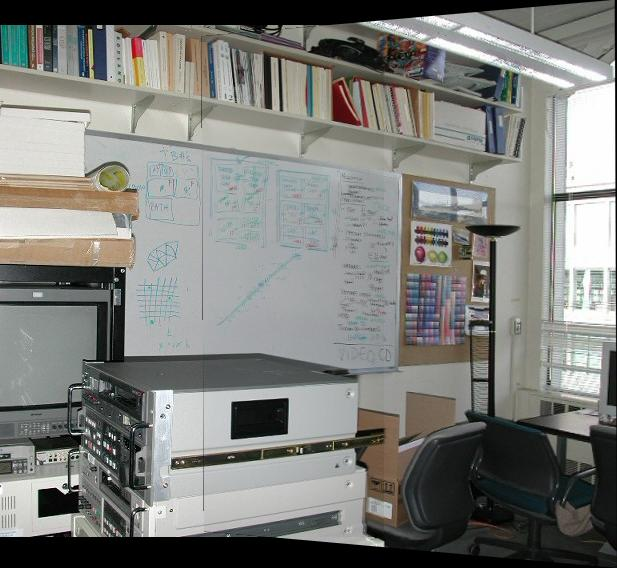
\includegraphics[width=\textwidth]{images/Part_5/Final_Panorama_set1.jpg}
        \caption{مجموعه اول: گسترش زاویه دید و اتصال موفق بافت‌ها}
    \end{subfigure}
    
    \vspace{0.6cm}
    \begin{subfigure}{0.65\textwidth}
        \centering
        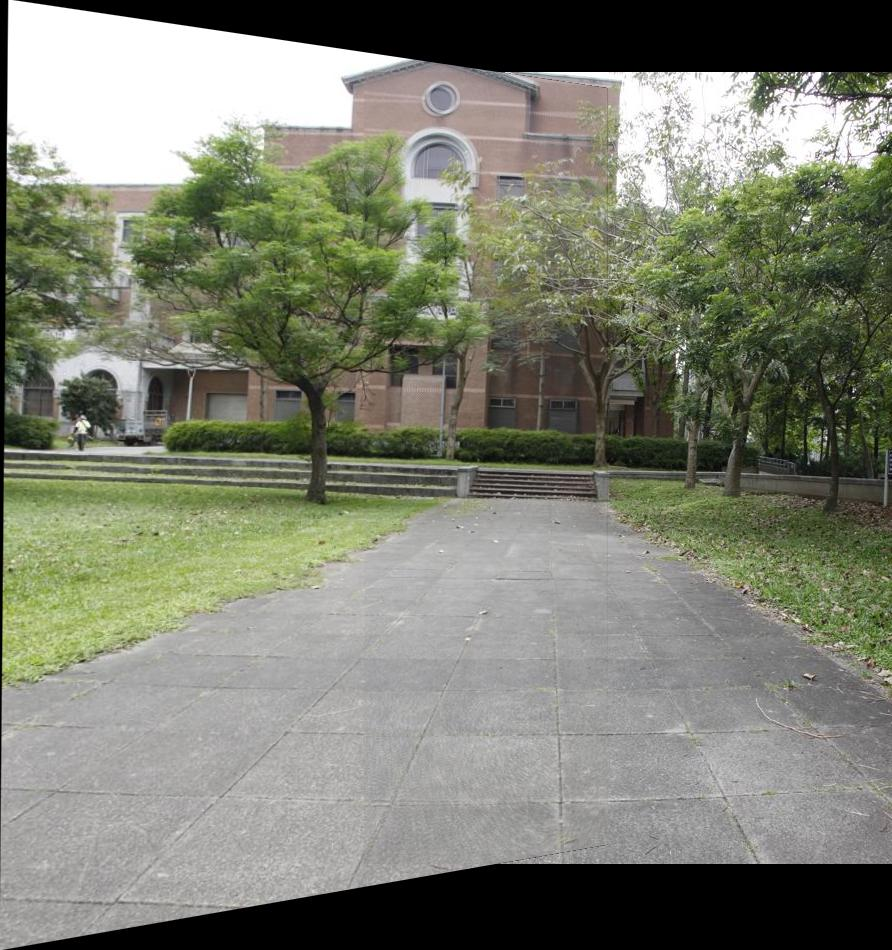
\includegraphics[width=\textwidth]{images/Part_5/Final_Panorama_set2.jpg}
        \caption{مجموعه دوم: ادغام نرم (\lr{Linear Blending}) بدون ایجاد خط درز}
    \end{subfigure}
    \caption{تصاویر سراسرنمای نهایی (\lr{Final Panoramic Images}) پس از ادغام و برش هوشمند (بخش اول)}
\end{figure}

% ------ انتقال به صفحه جدید ------
\newpage

% ------ بخش دوم تصاویر (صفحه دوم با پیوستگی شماره شکل) ------
\begin{figure}[h!]
    \ContinuedFloat
    \centering
    \begin{subfigure}{0.85\textwidth}
        \centering
        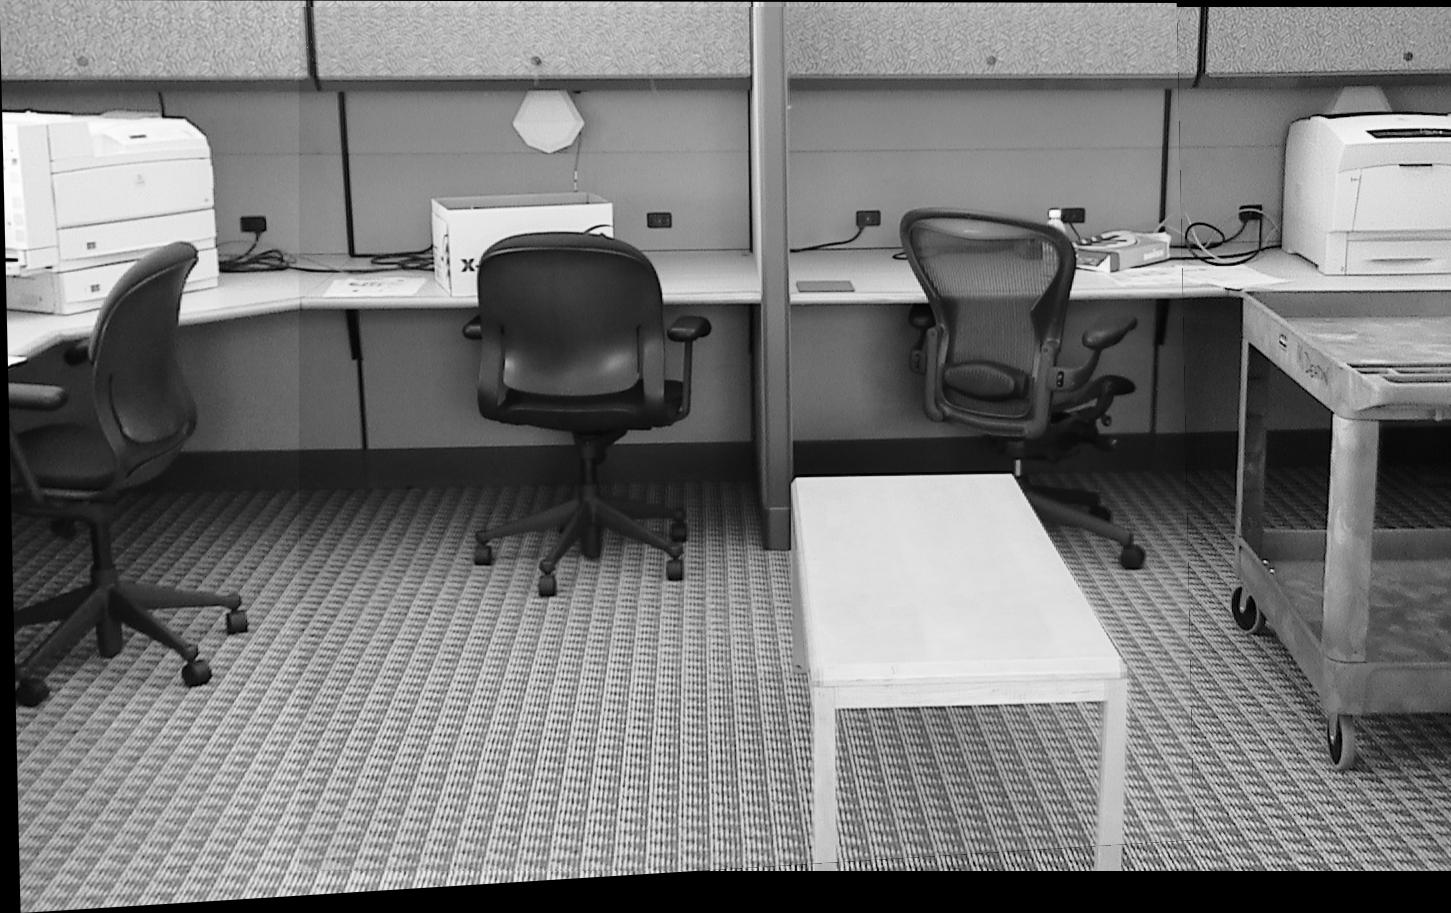
\includegraphics[width=\textwidth]{images/Part_5/Final_Panorama_set3.jpg}
        \caption{مجموعه سوم: حفظ کامل اطلاعات سمت چپ به کمک شیفت هندسی}
    \end{subfigure}
    \caption{تصاویر سراسرنمای نهایی (\lr{Final Panoramic Images}) پس از ادغام و برش هوشمند (ادامه)}
\end{figure}